\documentclass[ngerman]{article}
\synctex=1
\usepackage[utf8]{inputenc}
\usepackage{babel}
\usepackage{amsmath}
\usepackage{amssymb}
\usepackage{hyperref}
\usepackage{xcolor}
\usepackage[a4paper]{geometry}
\usepackage{siunitx}
\usepackage{graphicx}
\usepackage{bm}
%\usepackage{fourier}
\newtheorem{defi}{Definition}[section]
\newtheorem{satz}{Satz}[section]
\newtheorem{bsp}{Beispiel}[section]
% Kommentare beginnen mit dem Zeichen "%"

% Einstellung die verhindert, dass unschöne Rahmen um Links gezogen werden
\hypersetup{
    colorlinks = true, % false bedeutet Rahmen (nicht schön)
    linkcolor={red!20!black},
    citecolor={blue!50!black},
    urlcolor={blue!80!black},
}
% Syntax: \colorboxed[<color model>]{<color specification>}{<math formula>}
\newcommand*{\colorboxed}{}
\def\colorboxed#1#{%
  \colorboxedAux{#1}%
}
\newcommand*{\colorboxedAux}[3]{%
  % #1: optional argument for color model
  % #2: color specification
  % #3: formula
  \begingroup
    \colorlet{cb@saved}{.}%
    \color#1{#2}%
    \boxed{%
      \color{cb@saved}%
      #3%
    }%
  \endgroup
}
% Abkürzungen einführen (alphabetische Sortierung empfehlenswert):

\newcommand{\ad}{\mathrm{ad}}
% renew weil \d schon belegt ist
\renewcommand{\d}{\mathrm{d}} % aufrechtes d (für Differentialformen)
\newcommand{\NV}{{\cal N}\,}
\newcommand{\rang}{\mathrm{rang}}
\newcommand{\im}{\mathrm{im}}
\newcommand{\spann}{\mathrm{span}}
\newcommand{\R}{\mathbb{R}} % doppeltes R
\newcommand*{\pd}[3][]{\ensuremath{\frac{\partial^{#1} #2}{\partial #3}}}


% Hier beginnt das eigentliche Dokument
\begin{document}

%****************************Titelseite****************************************

%\onehalfspacing
\pagestyle{empty}

\begin{center}
	\Large \textbf{TECHNISCHE UNIVERSITÄT DRESDEN \\ \vspace{1.5cm} FAKULTÄT ELEKTROTECHNIK UND INFORMATIONSTECHNIK\\ \vspace{4cm}
 {\Huge Steuerung von Systemen mit örtlich verteilten Parametern}}\\
	\vspace{4cm}
	gehalten im SS 2018 \\ \vspace{1cm}
 \textbf{Institut für Regelungs- und Steuerungstheorie}\\
\vspace{2cm}

\end{center}
\newpage
\tableofcontents
%\numberwithin{equation}{section}
\setcounter{section}{1}
\pagestyle{headings}
\newpage
\section{Modellierung von Systemen mit verteilten Parametern}
\subsection{Modellierung in ortsfesten Koordinaten}
\label{sec:modortsfest}
\subsubsection{Bilanzgleichungen im $\R^3$}
\begin{itemize}
\item Medien mit fester Lage und Ausdehnung $\Omega \in \R^3$ (Berandung $\delta \Omega$) im Raum
\item Addressierung eines Punktes durch Ortsvektor $\bm{z}\in \Omega$
\item Bilanzierung der Speichergröße $S$ mit Dichtefunktion $s$ über beliebiges raumfestes Volumen $V \in \Omega$ mit Berandung $\delta \Omega$
\end{itemize}
Speichergrößenwert in V:
\begin{align}
\label{eq:speichergroesse}
S_V = \int_V s(\bm{z},t) \d V
\end{align}
Zeitableitung:
\begin{align}
\label{eq:diffspeichergroesse}
\dot{S}_V = \int_V \frac{\partial s(\bm{z},t)}{\partial t}\d V
\end{align}
Ursache der Änderung von $S_V$:
\begin{itemize}
\item Quellendichte $p$ im Inneren von $V$
\item Zustrom über den Rand (gerichtete Flussdichte $\bm{q}$
\end{itemize}
 \begin{align}
 \label{eq:ursache}
 \frac{dS_V}{dt} = \int_V p(\bm{z},t)dV - \int_{\delta V} \left\langle  \bm{q}(\bm{z},t),\bm{\nu}_{\delta V}(\bm{z})\right\rangle \d  \delta V
 \end{align}
Aus dem Integralsatz von Gauss folgt:
 \begin{align}
 \label{eq:satzvongauss}
  \int_{\delta V} \left\langle  \bm{q}(\bm{z},t),\bm{\nu}_{\delta V}(\bm{z})\right\rangle \d \delta V = \int_V \mathrm{div} \bm{q}(\bm{z},t) \d V
 \end{align}
 also:
 \begin{align*}
 \frac{dS_V}{dt} = \int_V p(\bm{z},t) - \mathrm{div} \bm{q}(\bm{z},t) \d V
 \end{align*}
 mit \eqref{eq:speichergroesse} und \eqref{eq:diffspeichergroesse}
 \begin{align}
 \label{eq:pdefinal}
 0 =  \int _V \left( \frac{\partial s(\bm{z},t)}{\partial t}-p(\bm{z},t)+\mathrm{div} \bm{q}(\bm{z},t) \right) \d V
 \end{align}
 Da Volumen beliebig muss der Integrand verschwinden
 \begin{align}
 0 = \frac{\partial s(\bm{z},t)}{\partial t}-p(\bm{z},t)+\mathrm{div} \bm{q}(\bm{z},t) 
 \end{align}
 \begin{itemize}
 \item Konkrete Aufgabnstellung definiert Zusammenhang zw. $s$ und $q$
\item Zusätzlich zu stellen: Randbedingungen zur pDgl.
\item Klassifikation der Randbedingungen: 
\subitem Vorgabe der Speichergröße auf $\delta \Omega \rightarrow $ Dirichlet
\subitem Vorgabe des Flusses auf $\delta \Omega \rightarrow $ Neumann
\subitem Funktionaler Zusammenhang von $s$ und $q$ auf $\delta \Omega \rightarrow$ gemischte RB
 \end{itemize}
 \subsubsection{Bilanzgleichungen im $\R^1$}
 \begin{itemize}
 \item Flussdichte $\bm{q}(\bm{z},t) \rightarrow$ Skalar $q(z,t) \in \R$
 \item Volumen $V \rightarrow$ Intervall $[a,b]$
 \item Randintegral \eqref{eq:satzvongauss} $\int_{\delta V} \left\langle  \bm{q}(\bm{z},t),\bm{\nu}_{\delta V}(\bm{z})\right\rangle \d  \delta V = q(b,t)-q(a,t) = \int_b^a \frac{\partial q(z,t)}{\partial z}\d z$
 \end{itemize}
 also statt \eqref{eq:pdefinal}
 \begin{align}
 \int_b^a \left( \frac{\partial s(z,t)}{\partial t}-p(z,t)+\frac{\partial q(z,t)}{\partial t} \right) \d z = 0
 \end{align}
 pDgl.:
 \begin{align}
 \frac{\partial s(z,t)}{\partial t}-p(z,t)+\frac{\partial q(z,t)}{\partial t}
 \end{align}
 Faustregel: Zu einer pDgl. $n$-ter Ordnung im Ort müssen $n$ unabhängige Randbedingungen vorgegeben werden.
 \subsection{Modellierung in materialfesten Koordinaten}
 \begin{itemize}
 \item deformierbare Medien in der Mechanik
 \item materialfestes Koordinatensystem 
 \subitem $\rightarrow$ Addressierung eines Materialpunktes $\bm{z}$ durch Ortsvektor $\bm{x}(\bm{z},t_0)$ in Referenzkonfiguration, die zue inem Zeitpunkt $t_0$ angenommen wird: $\bm{z}=\bm{x}(\bm{z},t_0)$
 \item im deformierten Zustand $\bm{z}\neq\bm{x}(\bm{z},t_0)$
 \item Bilanzierung in materialfesten Volumen ( Dichtefunktionen $p,s,\bm{q}$ müsssen in materialfesten Koordinaten gegeben sein)
 \item Gleichungen aus \ref{sec:modortsfest} gelten in materialfesten Koordinaten
 \end{itemize}
 \subsection{Modellierung in raumfesten Koordinaten durch Bilanzierung über materialfestem Volumen}
 \subsubsection{im $\R^3$}
 Ziel: Modellierung bewegter Medien in raumfestem Bezugssystem (z.B. Fluidmechanik)
 \begin{itemize}
  \item Addressierung eines Punktes $P$ des Kontinuums $\Omega$ durch den Ortsvektor $\bm{r}$ ine einer Referenzkonfiguration (Materialkoordinaten)
  \item Position von $P$ zum Zeitpunkt t (Raumkoordinaten): $\bm{z}(\bm{r},t) = \phi(\bm{r},t)$ 
 \end{itemize}

Annahme: $\phi$ ist zu jedem Zeitpunkt bezüglich $\bm{r}$ umkehrbar (jedem Raumpunkt entspricht eindeutig ein Matrialpunkt)
\begin{align*}
\bm{r} = \psi(\bm{z},t)
\end{align*}
Geschwindigkeit des Materialpunktes $P$:
\begin{align*}
\dot{\bm{z}}(\bm{r},t) = \frac{\partial \phi}{\partial t}(\bm{r},t)
\end{align*}
Zuordnung der Geschwindigkeiten zu einem Raumpunkt $\bm{z}$:
\begin{align*}
\bm{v}(\bm{z},t) := \dot{\bm{z}}(\psi(\bm{z},t),t)
\end{align*}
\begin{itemize}
\item Modellierung durch Bilanzierung einer Speichergröße $S_{V_t}$ (Dichte: $s(\bm{z},t)$) über ein materialfestes Volumen $V$, das zum Zeitpunkt $t$ das Volumen $V_t$ einnimmt:
\end{itemize}
\begin{align*}
S_{V_t} = \int_{V_t} s(\bm{z},t) \d V_t
\end{align*}
Integrationsgebiet $V_t$ nicht konstant! 

Deshalb wird die zeitliche Änderung von $S_{V_t}$ mit dem Transportsatz von Reynolds beschrieben:
\begin{align*}
\dot{S}_{V_t} = \int_{V_t} \frac{\partial s(\bm{z},t)}{\partial t}\d V_t + \int_{\delta V_t}s(\bm{z},t) \left\langle \bm{\nu}_{\delta V_t}(\bm{z},t),\bm{v}(\bm{z},t) \right\rangle \d \delta V_t
\end{align*}
mit der Notation aus \ref{sec:modortsfest} ergibt sich:
\begin{align}
\frac{\partial s(\bm{z},t)}{\partial t}-p(\bm{z},t)+\mathrm{div}\bm{q}(\bm{z},t)+\mathrm{div}\bm{s}(\bm{z},t)\bm{v}(\bm{z},t) = 0
\end{align}
\subsubsection{im $\R^1$}
\begin{figure}[ht]
	\centering
	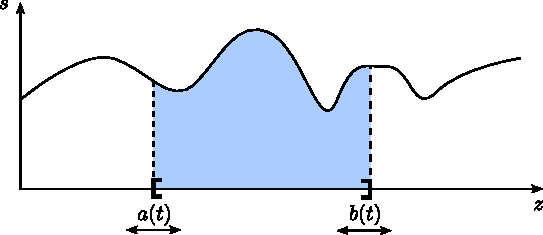
\includegraphics{img/bilanz1d}
	\label{fig:bilanz1d}
\end{figure}
\begin{itemize}
\item Wert der Bilanzgröße durch Integration über das mitbewegte Intervall $V_t=[a(t),b(t)]$
\end{itemize}
\begin{align*}
S_{V_t}=\int_{a(t)}^{b(t)}s(z,t)\d z
\end{align*}
Ableitung der Grenzen:
\begin{align*}
\frac{\partial a(t)}{\partial t} = v(a(t),t) \qquad \frac{\partial b(t)}{\partial t} = v(b(t),t)
\end{align*}
statt Anwendung des Transportsatzes von Reynolds
\begin{align*}
\frac{\d}{\d t}S_{V_t} = \frac{\d}{\d t}\int_{a(t)}^{b(t)}s(z,t)\d z &= s(b(t),t)\dot{b}(t)-s(a(t),t)\dot{a}(t)+\int_{a(t)}^{b(t)}\frac{\partial s(z,t)}{\partial t}\d z \\
&= s(b(t),t)v(b(t),t)-s(a(t),t)v(a(t),t)+\int_{a(t)}^{b(t)}\frac{\partial s(z,t)}{\partial t}\d z \\
&=\int_{a(t)}^{b(t)}\frac{\partial}{\partial z}v(z,t)s(z,t)\frac{\partial s(z,t)}{\partial t}\d z 
\end{align*}
mit der Notation aus \ref{sec:modortsfest} ergibt sich:
\begin{align}
\frac{\partial s(z,t)}{\partial t}-p(z,t)+\frac{\partial}{\partial z}(v(z,t)s(z,t)+q(z,t))= 0
\end{align}
\newpage
\section{Klassifikation partieller Differentialgleichungen}
\setcounter{equation}{0}
Erinnerung: Methoden der Charakteristiken zur Lösung pDgl.
\begin{bsp} 
Gesucht ist $x(z,t) \quad z,t,x \in \R$
\begin{align*} 
&(1+x)\frac{\partial x}{\partial t}-(1+z)\frac{\partial x}{\partial z} = z - t \\
\leftrightarrow&(1+x)\frac{\partial x}{\partial t}-(1+z)\frac{\partial x}{\partial z}  -z + t = 0
\end{align*}
Ansatz: $z=z(s)$, $t=t(s)$, $x=x(s)=x(z(s),t(s))$
Es gilt:
\begin{align*} 
&\frac{\d x}{\d t} = \frac{\partial x}{\partial z}\frac{\d z}{\d s} +\frac{\partial x}{\partial t}\frac{\d t}{\d s}  \\
\leftrightarrow & \frac{\partial x}{\partial z}\frac{\d z}{\d s} +\frac{\partial x}{\partial t}\frac{\d t}{\d s} - \frac{\d x}{\d t} = 0
\end{align*}
\textcolor{red}{Markieren in beiden Gleichungen, wass gleichgesetzt wird}

Offenbar muss gelten:
\begin{align*}
\frac{\d t}{\d s} &= 1+t \\
\frac{\d z}{\d s} &= -(1+z) \\
\frac{\d x}{\d s} &= z-t
\end{align*}
Dieses Gls. nennt man charakteristisches Dgl. System
Lösung (charakteristische Kurven):
\begin{align*}
t(s) &= C_1 e^s -1 \\
z(s) &= C_2 e^{-s} - 1 \\
x(s) &= C_3-C_2 e^{-s} - C_1 e^s \\
\end{align*}
Es gilt: 
\begin{align*}
e^s &= \frac{t+1}{C_1} = \frac{C_2}{z+1} \\
&\leftrightarrow (t+1)(z+1) = C_1C_2=:C \\
\end{align*}
ferner:
\begin{align*}
&x = C_3 - (z+1)-(t+1) \\
&x+z+t = C_3-2=: d \\
\end{align*}
Eine Lösung:
\begin{align*}
x(z,t)=-z-t+d \\
\end{align*}
Allgemein: $x = \phi((z+1)(t+1),x+z+t)$ ist Lösung mit beliebiger $\underbrace{C^1}_{\text{1-mal stetig diffbar}}$-Fkt. $: \phi:\R^2 \rightarrow \R$
\end{bsp}
\subsection{Charakteristika von Gleichungen erster Ordnung}
Ausgangspunkt:
\begin{align}
\label{eq:allgpde}
a(x(z,t),z,t)\frac{\partial x(z,t)}{\partial z}+b(x(z,t),z,t)\frac{\partial x(z,t)}{\partial t}=c(x(z,t),z,t)
\end{align}
Dabei ist $x$ eine Größe nach der aufgelöst werden muss.
Für eine beliebige Kurve
\begin{align*}
\Gamma: s \mapsto (z,t) = (a(s),b(s))
\end{align*}
wird eine Lösung von \eqref{eq:allgpde} vorgegeben:
\begin{align}
\label{eq:pdesolve}
x(a(s),b(s))=h(s)
\end{align}

\begin{figure}[ht]
	\centering
	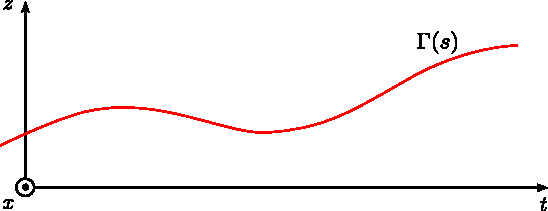
\includegraphics{img/charakteristik}
	\label{fig:charakteristik}
\end{figure}
Frage: Berechnung der Ableitungen $\frac{\partial x(z,t)}{\partial z}$ und $\frac{\partial x(z,t)}{\partial t}$ auf $\Gamma$ aus $h$ möglich?

Vorgehen: Differenzieren von \eqref{eq:pdesolve} nach $s$

\begin{align*}
\frac{\d h(s)}{\d s} = \frac{\partial x(z,t)}{\partial z}(\alpha(s),\beta(s))\alpha'(s)+\frac{\partial x(z,t)}{\partial t}(\alpha(s),\beta(s))\beta'(s)
\end{align*}
Zusammen mit \eqref{eq:allgpde} folgt:
\begin{align}
\label{eq:matrixpde}
\underbrace { \begin{pmatrix} a & b \\ \alpha ' & \beta ' \end{pmatrix} }_{ { \bm{C}} } \begin{pmatrix} \frac { \partial x }{ \partial z }  \\ \frac { \partial x }{ \partial t }  \end{pmatrix}=\begin{pmatrix} c \\ h' \end{pmatrix}
\end{align}
Kann nicht aufgelöst werden (Matrix nicht regulär), nennt man die Kurve $\Gamma$ charakteristisch.

Prüfung der Singularität von $\bm{C}$ wenn Zeilen linear abhängig sind
\begin{align}
\label{eq:singularitaetpruefung}
\alpha'= \frac{\d z}{\d s} = f_d a \big|_\Gamma \qquad \beta'= \frac{\d t}{\d s} = f_db \big|_\Gamma
\end{align}
mit der beliebigen Funktion $f_d$.
\begin{defi}
Eine nichttriviale Kurve $\Gamma:s\mapsto(\alpha(s),\beta(s)) \in \R^2$ heißt charakteristische Projektion zur pDgl. \eqref{eq:allgpde}, wenn \eqref{eq:singularitaetpruefung} mit einer beliebigen Funktion $f_d$ gilt.
\end{defi}
Charakteristiken:

Differenz der Zeilen von \eqref{eq:matrixpde} ergibt:
\begin{align*}
\frac{\d x}{\d s}\Big\rvert_\Gamma = h'= fc\big|_\Gamma
\end{align*}
Lösung der Kurve $\Gamma$ (entlang der Projektion) genügt der Dgl.
Es folgt mit \eqref{eq:singularitaetpruefung} das charakteristische Dgl.-System zu \eqref{eq:allgpde} ($f_d = 1,$ da beliebig):
\begin{align}
\label{eq:charkteristiken}
\frac{\d z}{\d s} = a \quad \frac{\d t}{\d s} = b \quad \frac{\d x}{\d s} = c
\end{align}
Lösungen $s \mapsto (t,z,x)$ des charakteristischen Systems \eqref{eq:charkteristiken} heißen charakteristische Kurven zu \eqref{eq:allgpde}.
\newpage
\subsection{Charakteristiken und Klassifikation von Gleichungssystemen 1. Ordnung}
\label{sec:3.2}
Ausgangspunkt: 
\begin{align}
\label{eq:6}
\bm{A}(\bm{x}(z,t))\frac{\partial \bm{x}(z,t)}{\partial z}+\bm{B}(\bm{x}(z,t))\frac{\partial \bm{x}(z,t)}{\partial t} = \bm{c}(\bm{x}(z,t),z,t)
\end{align}
\begin{align*}
\label{eq:6'}
\textrm{kurz: } \bm{A}\frac{\partial \bm{x}(z,t)}{\partial z}+\bm{B}\frac{\partial \bm{x}(z,t)}{\partial t}=\bm{c} \tag{6'}
\end{align*}
Annahme:
\begin{align*}
\det(\mu \bm{A}+ \nu \bm{B}) \neq 0 
\end{align*}
$\mu, \nu \in \R \rightarrow$ Regularität von \eqref{eq:6}.
Charakteristiken: 
Eine Kurve $\Gamma:s \mapsto (\alpha(s),\beta(s))=(z,t)$ ist eine charakteristische Projektion zu \eqref{eq:6}, wenn es nicht möglich ist aus
\begin{align} 
\label{eq:7}
\bm{x}(\alpha(s),\beta(s))=:\bm{h}(s)
\end{align}
die Ableitungen $\frac{\partial \bm{x}(z,t)}{\partial z}, \frac{\partial \bm{x}(z,t)}{\partial t}$ auf $\Gamma$ zu berechnen.
Differenzieren von \eqref{eq:7}:
\begin{align*}
\frac{\partial \bm{x}(\alpha(s),\beta(s))}{\partial z}\alpha'(s)+\frac{\partial \bm{x}(\alpha(s),\beta(s))}{\partial t}\beta'(s)=\bm{h}'(s)
\end{align*}
ergibt mit \eqref{eq:6'}
\begin{subequations}
\begin{align}
\bm{A}\frac{\partial \bm{x}}{\partial z}+\bm{B}\frac{\partial \bm{x}}{\partial t} =\bm{c}
\end{align}
\begin{align}
\alpha'\frac{\partial \bm{x}}{\partial z}+\beta'\frac{\partial \bm{x}}{\partial t} =\bm{h}'
\end{align}
\end{subequations}
Beobachtung: $\alpha', \beta'$ können nicht verschwinden.

Fall 1: $\alpha' \neq 0$
$(8a)\alpha-(8b)\bm{A}:(\alpha'\bm{B}-\beta'\bm{A})\frac{\partial \bm{x}}{\partial t}=\alpha'\bm{c}-\bm{A}\bm{h}'$

Fall 2: $\beta' \neq 0$
$(8a)\beta-(8b)\bm{B}:(\beta'\bm{A}-\alpha'\bm{B})\frac{\partial \bm{x}}{\partial z}=\beta'\bm{c}-\bm{B}\bm{h}'$

Damit $\frac{\partial \bm{x}}{\partial z}$ bzw. $\frac{\partial \bm{x}}{\partial t}$ nicht bestimmt werden können, muss gelten:
\begin{align}
\label{eq:9}
\det(\beta'\bm{A}-\alpha'\bm{B}) \overset{!}{=} 0
\end{align}
Für Charakterisierung wird folgender Spezialfall betrachtet:
Untersuchung der Kurve $s \mapsto (0,s)$. Diese Kurve soll keine Charakteristik sein.

\begin{figure}[ht]
	\centering
	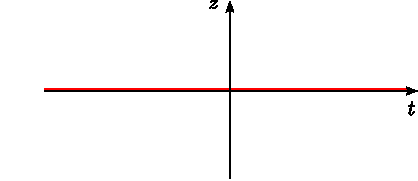
\includegraphics{img/keinecharakteristik}
	\label{fig:keinecharakteristik}
\end{figure}

Dann folgt für Charakteristik $\alpha(s) \neq 0$
$\underbrace{\Rightarrow}_{\eqref{eq:9}} $
Multiplikation von \eqref{eq:6} mit $\bm{A}^{-1}$
\begin{align*}
\pd{\bm{x}}{z}=-\underbrace{\bm{A}^{-1}\bm{B}}_{\bm{B}^*} \pd{\bm{x}}{t}+\underbrace{\bm{A}^{-1}\bm{c}}_{\bm{c}^*}
\end{align*}
aus \eqref{eq:9} folgt: 
\begin{align*}
\det(\beta'\bm{I}_n-\alpha'\bm{B}^*)=0
\end{align*}
da $a'\neq0$
\begin{align*}
\det\Big(\underbrace{\frac{\alpha'}{\beta'}}_{\lambda}\bm{I}_n-\bm{B}^*\Big)=0 \textrm{ mit } &\beta(s) = t(s) \quad \beta'=\frac{dt}{ds} \\ &\alpha(s) = z(s) \quad \alpha'=\frac{dz}{ds}
\end{align*}
$\lambda = \frac{dt}{dz}$ sind somit die Eigenwerte von $\bm{B}^*=\bm{A}^{-1}\bm{B}$.
Klassifikation:
\begin{itemize}
\item alle Eigenwerte sind komplex $\rightarrow$ elliptisches System (z.B. örtlich 2-dim stationäre Probleme, d.h. $t$ ist 2. Ortskoordinate)
\item alle Eigenwerte reel, zu jedem Eigenwert existiert ein Eigenvektor, $\bm{B}^*$ ist diagonalisierbar $\rightarrow$ hyperbolisches System
\item $\bm{B}^*$  besitzt nur einen reellen Eigenvektor $\rightarrow$ parabolisches System
\end{itemize}

parabolisch/hyperbolisch: dynamische Phänomene

Mischtypen möglich, physikalisch sinnvoll: hyperb.-parab.

\subsection{Klassifikation und Charakteristiken von Gleichungen 2. Ordnung}
Ausgangspunkt: Skalare pDgl. 2. Ordnung (jetz: Gl. 10)
\begin{align}
\label{eq:10}
a \frac{\partial^2 x}{\partial^2 z} + 2b \frac{\partial^2x}{\partial z\partial t} + c \frac{\partial^2 x}{\partial t^2} = d
\end{align}
($a,b,c,d$ hängen von $z,t,x,\frac{\partial x}{\partial z},\frac{\partial x}{\partial t}$ ab)

Vorgabe von $x,\frac{\partial x}{\partial z},\frac{\partial x}{\partial t}$ auf 
\begin{align*}
\Gamma:\R \rightarrow \R \times \R \textrm{ mit } s \mapsto (\alpha(s),\beta(s))=(z,t)
\end{align*}
mit 
\begin{subequations}
\begin{align}
\alpha(s),\beta(s)) = h(s) \label{eq:11a}\\
\frac{\partial x}{\partial z}(\alpha(s),\beta(s))=\phi(s) \label{eq:11b}\\
\frac{\partial x}{\partial t}(\alpha(s),\beta(s))=\psi(s) \label{eq:11c}
\end{align}
\end{subequations}
Frage: Wann können  $\frac{\partial^2 x(z,t)}{\partial z^2},\frac{\partial^2 x(z,t)}{\partial z \partial t}=\frac{\partial^2 x(z,t)}{\partial z \partial z},\frac{\partial^2 x(z,t)}{\partial t^2}$ auf $\Gamma$ aus $h,\phi, \psi$ berechnet werden?
Es gilt:
\begin{align*}
\eqref{eq:11a} \quad h'(s) &= \pd{\bm{x}}{z} \alpha' + \pd{\bm{x}}{t}\beta' = \varphi(s)\alpha'(s) + \psi(s)\beta'(s) \\
\eqref{eq:11b} \quad \varphi'(s) &= \pd[2]{\bm{x}}{z} \alpha' + \pd[2]{\bm{x}}{z\partial t}\beta' \\
\eqref{eq:11c} \quad \psi'(s) &= \pd[2]{\bm{x}}{z \partial t} \alpha' + \pd[2]{\bm{x}}{^2 t}\beta' \\
\end{align*}
aus \eqref{eq:11b}, \eqref{eq:11c} und \eqref{eq:10} folgt:
\begin{align}
\label{eq:12}
\underbrace{\begin{pmatrix}
a & 2b & c \\
\alpha' & \beta' & 0 \\
0 & \alpha'& \beta'
\end{pmatrix}}_{\bm{M}}\begin{pmatrix}
\pd[2]{\bm{x}}{z^2} \\ \pd[2]{\bm{x}}{z\partial t} \\ \pd[2]{\bm{x}}{t^2}
\end{pmatrix} =
\begin{pmatrix}
d \\ \varphi' \\ \psi'
\end{pmatrix}
\end{align}
charakteristisch $\Rightarrow \det(\bm{M})=0$
\begin{align}
\Rightarrow a \beta'^2 - 2b \alpha' \beta' + c \alpha'^2 = 0
\end{align}
Spezialfall (wie in \ref{sec:3.2}) Betrachtung von Charakteristiken mit $\alpha'(s) \neq 0$ und zusätzlich $z = \alpha(s)=s$
\begin{align*}
\Rightarrow &a \beta' - 2b \alpha' \beta' + c \alpha'^2 = 0 | \cdot \frac{1}{\alpha'}(=1) \\
&a \frac{\beta'^2}{\alpha'^2} - 2b \frac{\beta'}{\alpha'} + c = 0 \\
&a\lambda^2-2 b \lambda + c = 0 \\
&\lambda_{1/2}=\frac{b}{a} \pm \frac{\sqrt{b^2-ac}}{a}  
\end{align*}
\begin{align*}
&b^2-ac >0 \quad &\textrm{reelle Lsg., hyperbolisch} \\
&b^2-ac <0 \quad &\textrm{konj. kompl. Lsg., elliptisch} \\
&b^2=ac \quad &\textrm{parabolisch}
\end{align*}
\newpage
\section{Steuerungsentwurf}
\subsection{Motivation Steuerungsentwurf}
$\Rightarrow$ Folien

\subsection{(Differentielle) Flachheit konzentriertparametrischer Systeme}
Modell Feder-Masse-Schwinger 
\begin{align*}
m\ddot{x}(t)+\sigma \frac{x(t)}{l} = u(t)
\end{align*}
Stellgröße $u$ ergibt sich direkt aus der vertikalen Auslenkung $x$ und deren zweiter Ableitung $\ddot{x}$.
Damit ist $x$ ein flacher Ausgang $y$. Mithin gilt für die Steuerung:
\begin{align*}
u_{ref}(t) =  m \ddot{y}_{ref}(t) +\frac{\sigma}{l}y_{ref}(t)
\end{align*}
Trajektorienplanung für $y_{ref}: t \mapsto y_{ref}(t)$ muss zweimal stetig differenzierbar sein.
\begin{bsp}
\begin{align*}
y_{ref}(t) = \begin{cases} y_0 \quad t<0 \\ y_0 +(y_1-y_0)\varphi(t/t^*) \quad t\in [0,t^*] \\ y_1 \quad t>t^* \end{cases}
\end{align*}
mit $\varphi(\tau) = 10 \tau^3-15\tau^4+6\tau^5$ für Übergang von $y_0$ auf $y_1$, innerhalb der Zeit $t^*$.

\textcolor{red}{Abbildung fehlt}

Reglerentwurf: 
\begin{enumerate}
\item Vorgabe einer Fehlerdynamik:

\[\ddot{\tilde{y}}(t)+k_1\dot{\tilde{y}}(t)+k_0 \tilde{y}(t)= 0, \quad\tilde{y}=y-y_{ref}\]

\[\ddot{y}=\ddot{y}_{ref}-k_1\dot{\tilde{y}}-k_0 \tilde{y}\]

\item ins Modell eingesetzt:
\begin{align*}
u=m(\ddot{y}_{ref}-k_1\dot{\tilde{y}}-k_0 \tilde{y})+\frac{\sigma}{l}y
\end{align*}
\end{enumerate}
\end{bsp}
Verteiltparametrisches Beispiel:

\begin{bsp}Schwingende Saite (Modellbildung s. Folie)
\begin{align*}
\rho\pd[2]{x}{t^2}(z,t)-\sigma\pd[2]{x}{z^2}(z,t) = 0 \\
\textrm{mit RB: } x(0,t) = 0, \quad \sigma \pd{x}{z}(l,t)=u(t)
\end{align*}
\begin{itemize}
\item[] Flacher Ausgang: $y(t) = \pd{x}{z}(0,t)$ aus Grenzübergang Modellbildung (s. Folie)

\item[] Weiteres Vorgen: Wenn $y$ bekannt ist, können $x(0,t)$ (aus RB) und $\pd{x}{z}(0,t)$ (aus Def. von $y$) berechnet werden.

\item[] Probleme:

\item Rekursion wie im konzentriertparametrischen Fall zur Berechung der werte am rechten Rand $(z=l)$ nicht möglich
\item stattdessen: Berechnung der Lösung der pDgl. aus bekannten Randtrajektorien für $t\mapsto\,x(0,t)$ und $t\mapsto\,\pd{x}{z}(0,t)$ nötig.
\item[$\Rightarrow$] Cauchy'sche Randwertaufgabe (sämtliche RB am gleichen Rand vorgegeben)
\item [$\Rightarrow$] Lösung der Randwertaufgabe und Auswertung der physikalischen Randbedingungen liefert Stellgrößenverlauf.
\end{itemize}
\end{bsp}
Thema im Folgenden: Transformation einer gegebenen RWA auf eine Cauchy'sche RWA durch Einführung eines flachen Ausgangs.

\subsection{Flacher Ausgang für eine Klasse von Randwertaufgaben (RWA)}
\setcounter{equation}{0}
Ausgangspunkt: $n$ pDgl. 1. Ordnung bezüglich $z$
\begin{align}
&\pd{\bm{x}}{z}(z,t) = \bm{f}(\bm{x}(z,t),\ddot{\bm{x}}(z,t),\ddot{\bm{x}}(z,t),...) \\
\hat{=}&\pd[n]{x}{z^n}(z,t)=f\Big(x(z,t),\pd{x}{z}(z,t),...,\pd[n-1]{x}{z^{n-1}}(z,t),\dot{x}(z,t),\ddot{x}(z,t),...\Big) \tag{1'}
\end{align}
Randbedingungen:
Modell $n$-ter Ordnung benötigt $n$ Randbedingungen (RB) 
\begin{enumerate}
\item vollständig gesteuerte RB 
\item[] o.B.d.A. bei $z=0$: 
\item[] $m$ dieser RB mit $m$ Stelleingriffen in $\bm{u}=(u_1,...,u_m)$ bei z=0:
\item[] $\bm{R}_0(\bm{u}(t),\bm{x}(0,t),\dot{\bm{x}}(0,t,),...)=0$ mit
 \[\bm{R}_0 = (R_{0,1},....,R_{0,m})^\textrm{T} \tag{2a} \label{eq:4-2a}\]können nach $\bm{u}$ aufgelöst werden, dh. $\rang(\pd{\bm{R}_0}{\bm{u}})=m$
\item[]Interpretation: $\bm{x}(0,t)$ ist flacher Ausgang des Systems \eqref{eq:4-2a}, denn $\bm{u}$ lässt sich aus $\bm{x}(0,t)$ und dessen Ableitungen integrallos berechnen.
\item vollständig differentiell paramterierbare RB 
\item[] o.B.d.A. bei $z=l$:
\item[] $n-m$ RB bei $z = l$ 
\item[] $\bm{R}_l(\bm{x}(l,t),\dot{\bm{x}}(l,t,),...)=0$ mit
 \[\bm{R}_l = (R_{l,1},....,R_{l,n-m})^\textrm{T} \tag{2b} \label{eq:4-2b}\] können nach $\bm{x}$ aufgelöst werden, dh. $\rang(\pd{\bm{R}_l}{\bm{x}})=n-m$
 \item[] Annahme: es existiert ein $\bm{y}(t)=(y_1(t),...,y_{m}(t))^\textrm{T}$ mit 
 \item[] \[\bm{y}(t) = \bm{g}\Big( \bm{x}(l,t),\dot{x}(l,t),...\Big) \tag{3} \label{eq:4-3}\]
 \item[] sodass gilt:
 \item[] \[\bm{x}(l,t) = \bm{h}\Big( \bm{y}(t),\dot{y}(t),...\Big)\tag{4} \label{eq:4-4}\]
 \item[] Interpretation $\bm{y}$ ist flacher Ausgang des konzentriertparametirischen Systems \eqref{eq:4-2b}
\end{enumerate}
\textcolor{red}{Abbildung fehlt}
\newpage
\subsection{Lösung der Cauchy'schen Randwertaufgabe für hyperbolische Systeme}
\setcounter{equation}{4}
Ausgangspunkt:
\begin{align}
\pd{\bm{x}}{z}(z,t)+\bm{B}(z)\pd{\bm{x}}{t}(z,t) = \bm{C}(z)\bm{x}(z,t)  \label{eq:4-5}
\end{align}
mit $\bm{x}(z,t) \in \R^n$ und hyperbolisch, da EW von $\bm{B}(z)$ reell und verschieden.
\\\\
Ziel: Berechnung er Lösung $(z,t)\mapsto\bm{x}(z,t)$ aus bekanntem Verlauf $t\mapsto\bm{x}(z_0,t)$ (z.B. $z_0=l$)
\\\\
Erinnerung: Eigenwerte $\lambda_1(z),...,\lambda_n(z)$ der Matrix $\bm{B}(z)$ mit $z=[0,l]$ entprechen Anstiegen der $\underbrace{\textrm{Charakteristiken}}_{\textrm{char. Projektion}}$, da System hyperbolisch
\\\\
Spannen die Eigenvektoren $\bm{r}_1(z),...,\bm{r}_n(z)$ von $\bm{B}(z)$ den $\R^n$ auf und $\bm{B}(z)$ ist mittels $\bm{T}=(\bm{r}_1(z),...,\bm{r}_n(z))$ diagonalisierbar:
\begin{align*}
\bm{\Lambda}(z)=\bm{T}^{-1}(z)\bm{B}(z)\bm{T}(z) = \begin{pmatrix}
\lambda_1(z) & & 0 \\ & \ddots & \\ 0 & & \lambda_n(z)
\end{pmatrix}
\end{align*}
Transformation von \eqref{eq:4-5} auf hyperbolische Normalform durch Wechsel der abhängigen Veränderlichen
\begin{align*}
\colorboxed{red}{\bm{x}(z,t) = \bm{T}(z)\tilde{\bm{x}}(z,t)}
\end{align*}
Einsetzen in \eqref{eq:4-5} liefert die hyperbolische Normalform
\begin{align*}
&\bm{T}(z)\pd{\tilde{\bm{x}}}{z}(z,t)+\pd{\bm{T}(z)}{z}\tilde{\bm{x}}(z,t)+\bm{B}(z)\bm{T}(z)\pd{\tilde{\bm{x}}}{t}(z,t) = \bm{C}(z)\bm{T}(z)\tilde{\bm{x}}(z,t) \\
\Leftrightarrow \quad &\pd{\tilde{\bm{x}}}{z}(z,t)+\bm{T}^{-1}(z)\pd{\bm{T}(z)}{z}\tilde{\bm{x}}(z,t)+\underbrace{\bm{T}^{-1}(z)\bm{B}(z)\bm{T}(z)}_{=:\bm{\Lambda}(z)}\pd{\tilde{\bm{x}}}{t}(z,t) = \bm{T}^{-1}(z)\bm{C}(z)\bm{T}(z)\tilde{\bm{x}}(z,t) \\
\Leftrightarrow \quad & \pd{\tilde{\bm{x}}}{z}(z,t) + \bm{\Lambda}(z)\pd{\tilde{\bm{x}}}{t}(z,t)=\underbrace{\left(\bm{T}^{-1}(z)\bm{C}(z)\bm{T}(z)-\bm{T}^{-1}(z)\right)}_{=:\tilde{\bm{C}}}\tilde{\bm{x}}(z,t)
\end{align*}
\begin{align}
\Leftrightarrow \quad \colorboxed{red}{\pd{\tilde{\bm{x}}}{z}(z,t) + \bm{\Lambda}(z)\pd{\tilde{\bm{x}}}{t}(z,t)= \tilde{\bm{C}}\tilde{\bm{x}}(z,t)}
\end{align}
schön, weil
\begin{align*}
& \tilde{x}_1'+\lambda_1\dot{\tilde{x}}_1=\tilde{c}_1^{\mathrm{T}}\tilde{\bm{x}} & \tilde{c}_i^{\mathrm{T}} \quad i\textrm{-te Zeile von }\tilde{\bm{C}}\\
& \tilde{x}_2'+\lambda_2\dot{\tilde{x}}_2=\tilde{c}_2^{\mathrm{T}}\tilde{\bm{x}} \\
& \qquad \vdots \\
& \tilde{x}_n'+\lambda_n\dot{\tilde{x}}_n=\tilde{c}_n^{\mathrm{T}}\tilde{\bm{x}}
\end{align*}
Charakteristik durch $(z_0,t_0)$:
\begin{align}
\colorboxed{red}{z\mapsto t_i(z;z_0)+t_0 \quad \mathrm{mit} \quad \frac{\d t_i}{\d z}(z;z_0) = \lambda_i(z)}
\end{align}
Ableitung von $\tilde{\bm{x}}_i$ $i=1,...,n$ entlang der zugehörigen Charakteristik durch $(z_0,t_0)$
\begin{align}
\pd{\tilde{x}_i}{z}(z,t_i(z;z_0)+t_0)+\lambda_i(z)\pd{\tilde{x}_i}{t}(z,t_i(z;z_0)+t_0) = \tilde{c}_i^{\textrm{T}}(z)\tilde{x}_i(z,t_i(z;z_0)+t_0)-\tilde{x}_i(z_0,t_0)
\end{align}
Integration $\int_{z_0}^z$ liefert:
\begin{align*}
\tilde{x}_i(z,t_i(z;z_0)+t_0)-\tilde{x}_i(z_0,t_0) = \int_{z_0}^z\tilde{c}_i^{\textrm{T}}(\xi)\tilde{x}_i(\xi,t_i(\xi;z_0)+t_0)-\tilde{x}_i(z_0,t_0)\d \xi
\end{align*}
da $t=t_i(z;z_0)+t_0$
\begin{align}
\label{eq:4-9}
\tilde{x}_i(z,t)-\tilde{x}_i(z_0,t-t_i(\xi;z_0)) = \int_{z_0}^z\tilde{c}_i^{\textrm{T}}(\xi)\tilde{x}_i(\xi,t)-\tilde{x}_i(z_0,t_0)\d \xi
\end{align}
\begin{satz}(ohne Beweis)
Das System \eqref{eq:4-9} von Integralgleichungen besitzt für beliebige beschränkte Randtrajektorien $t \mapsto \tilde{x}_i(z_0,t)$ eine eindeutige Lösung $(z,t) \mapsto \tilde{\bm{x}}(z,t)$. 
\end{satz}
Mit $\bm{x}(z,t)=\bm{T}(z)\tilde{\bm{x}}(z,t)$ folgt die Lösung der Cauchyschen Randwertaufgabe.

Numerische Lösung durch Diskretisierung des Integrals (Euler-Schema)
\begin{enumerate}
\item Zerlegung von $[0, l]$ in $N+1$ Intervalle $[z_k,z_{k+1}]$ der Länge $\Delta z$ \[\tilde{x}_i(z_{k+1},t)-\tilde{x}_i(z_{k},t-t_i(z_{k+1};z_k)) = \int_{z_k}^{z_{k+1}}\tilde{c}_i^{\textrm{T}}(\xi)\tilde{\bm{x}}(\xi,t-t_i(z_{k+1};\xi))\d \xi \]
\item Approximation $t_i(z_{k+1};z_k) \approx \Delta z \lambda_i(z)$ \[ \int_{z_k}^{z_{k+1}}\tilde{c}_i^{\textrm{T}}(\xi)\tilde{\bm{x}}(\xi,t-t_i(z_{k+1};\xi))\d \xi \approx \Delta z \tilde{c}_i^{\textrm{T}}(z_k)\tilde{\bm{x}}(z_k,t-t_i(z_{k+1},z_k)) \]
\begin{align}
\Rightarrow \tilde{x}_i(z_{k+1},t) = \tilde{x}_i(z_k,t-\Delta z \lambda_i(z_k)) + \Delta z \tilde{c}_i^{\textrm{T}}(z_k)\tilde{\bm{x}}(z_k,t-\Delta z \lambda_i(z_k))
\end{align}
\end{enumerate}
Spezialfall: $\tilde{c}_i^{\textrm{T}}=0$ Lösung ergibt sich durch eien Zeitverschiebung der Randtrajektorie (Totzeiten, Prädiktion)
\begin{bsp}{Elektrische Übertragungsleitung}
\begin{align*}
\pd{u}{z}(z,t)+L\pd{i}{t}(z,t)+Ri(z,t)&=0 \\
\pd{i}{z}(z,t)+C\pd{u}{t}(z,t)+Gu(z,t)&=0
\end{align*}
mit $\bm{x}(z,t)=\begin{pmatrix}
u(z,t) \\ i(z,t)
\end{pmatrix}$
\begin{align*}
\pd{\bm{x}}{z}(z,t)+\bm{B}\pd{\bm{x}}{t}(z,t)+\bm{C}\bm{x}(z,t)&=0
\end{align*}
mit $\bm{B}=\begin{pmatrix}
0 & L \\ C & 0
\end{pmatrix}$ und $\bm{C}=\begin{pmatrix}
0 & R \\ G & 0
\end{pmatrix}$
\begin{itemize}
\item[] Vorgabe $\bm{x}(z_0,t) =:\bm{x}_0(t)$
\item[] gesucht: $\bm{x}(0,t) =: u_0(t)$
\item[] Eigenwerte von $\bm{B}:\lambda_1 = \tau \quad \lambda_2 = -\tau$ mit $\tau = \sqrt{LC}$
\item[] Eigenvektoren von $\bm{B}:\bm{r}_1 = \begin{pmatrix}\sqrt{L} \\ \sqrt{C}\end{pmatrix} \quad \bm{r}_2 = \begin{pmatrix}\sqrt{L} \\ -\sqrt{C}\end{pmatrix} $
\item[] Transformation: $\bm{x}(z,t)=\bm{T}(z)\tilde{\bm{x}}(z,t)$ \newline mit  $\bm{T}(z) = \begin{pmatrix}\sqrt{L} &\sqrt{L} \\ \sqrt{C}&-\sqrt{C}\end{pmatrix}$ und $\bm{T}^{-1}(z) =\frac{1}{2\sqrt{LC}} \begin{pmatrix}\sqrt{C} &\sqrt{L} \\ \sqrt{C} &-\sqrt{L}\end{pmatrix}$
\item[] hyperbolische Normalform: \[ \pd{\tilde{\bm{x}}}{z}(z,t)+\tau\begin{pmatrix}1 & 0 \\ 0 & -1\end{pmatrix}\pd{\tilde{\bm{x}}}{t}=\frac{\tau}{2}\begin{pmatrix}-\alpha \tilde{x}_1+\beta\tilde{x}_2 \\ -\beta \tilde{x}_1+\alpha\tilde{x}_2\end{pmatrix} \] 
\[\alpha=\frac{R}{L}+\frac{G}{C} \quad \beta = \frac{R}{L}-\frac{G}{C} \]
\item[] Charakteristiken
\begin{align*}
(z_0,t_0) &\mapsto t_1(z;z_0)+t_0 \quad \mathrm{mit} \quad \frac{\d t_1}{\d z}(z;z_0)=\tau \\
(z_0,t_0) &\mapsto t_2(z;z_0)+t_0 \quad \mathrm{mit} \quad \frac{\d t_2}{\d z}(z;z_0)=-\tau \\
\end{align*}
auf den Charakteristiken gilt: 
\begin{align*}
\tilde{x}_1(z,t) = \tilde{x}_1(z_0,t-\tau(z-z_0))+\int_{z_0}^z\left(-\alpha\tilde{x}_1(\xi,t-\tau(z-\xi))+\beta\tilde{x}_2(\xi,t-\tau(z-\xi))\right) \\
\tilde{x}_2(z,t) = \tilde{x}_2(z_0,t+\tau(z-z_0))+\int_{z_0}^z\left(-\beta\tilde{x}_1(\xi,t+\tau(z-\xi))+\alpha\tilde{x}_2(\xi,t+\tau(z-\xi))\right)
\end{align*}
\end{itemize}
\end{bsp}
\newpage
\subsection{Lösung der Cauchy'schen Randwertaufgabe für parabolische Systeme}
\subsubsection{Mathematische Vorbereitungen}
$\Gamma$-Funktion: Verallgemeinerung der Fakultät für nicht ganzzahlige Argumente.

$\Gamma(i+1)=i! \quad i \in \mathbb{N}$ genügt der Funktionalgleichung:
\begin{align*}
\Gamma(x+1)=x\Gamma(x) \qquad \Gamma(1)=1
\end{align*}
\begin{defi} \textcolor{red}{Gevrey-Klasse} und \textcolor{red}{-Ordnung}. Die Funktion $f$ sei auf dem Intervall $\Omega \in \R$ definiert und dort beliebig oft differenzierbar. Dann gehört $f$ auf $\Omega$ zur kleinen Gevrey-Klasse $G_\alpha(\mathcal{I})$ der Ordnung $\alpha$, wenn zu jedem $\gamma>0$ eine Konstante $M$ derart existiert, dass gilt:
\begin{align*}
\sup_{t\in\mathcal{I}}{\pd[i]{f}{t^i}(t)<M\gamma^i\Gamma(\alpha i+1)}
\end{align*}
(alle Ableitungen für alle $t$ dürfen die Schranke (rechte Seite) nicht überschreiten)
\end{defi}
\begin{bsp}
\begin{align*}
\varphi_\gamma =  \begin{cases}0 & t<0 \\ \frac{1}{2}\left(1+\tanh\left(\frac{2t-1}{(4t(1-t))^\sigma}\rigt)\right) & t \in[0,1] \\1 &t>1 \end{cases}
\end{align*}
gehört zur kleinen Gevrey-Klasse der Ordnung $\alpha$ für $\sigma>\frac{1}{\alpha-1}$

Bei Interpolation treten in den Ableitungen bestimmter Ordnung in den Randpunkten Sprünge auf. Hier muss aber auch bei der $\infty.$ Ableitung kein Sprung sein.
\end{bsp}
\subsubsection{Existenz der Lösung}
Ausgangspunkt: homogenes lineares pDgl-System aus $n$ Gleichungen 1. Ordnung
\begin{align}
\pd{\bm{x}}{z}(z,t)+\bm{B}(z)\pd{\bm{x}}{t}(z,t) = \bm{C}(z)\bm{x}(z,t)  \quad \bm{x} \in \R^n \label{eq:4-11}
\end{align}
Ziel: Berechnung der Lösung $(z,t)\mapsto\bm{x}(z,t)$ aus bekanntem Verlauf $t\mapsto \tilde{x}(z_0,t)$ mit bspw. $z_0=l$

Annahme: $\bm{B}$ hat nur einen Eigenwert $\lambda=0$ der algebraischen Vielfachheit $n$ 

$\Rightarrow$ parabolisches System

geometrische Vielfachheit des Eigenwertes $\lambda$ sei $M=n-rang(\bm{B})$ 

$\Rightarrow$ $M$ Eigenvektoren zur Matrix $\bm{B}$

Folge: Es existiert eine matrixwertige Funktion
\begin{align*}
z\mapsto\bm{T}(z) \quad \bm{J}(z)=\bm{T}^{-1}(z)\bm{B}(z)\bm{T}(z)
\end{align*}
mit $\bm{J}$ in Jordan-Normalform

\begin{satz}\eqref{eq:4-11} genügen den obigen Annahmen. Sei $\hat{m}$ die maximale in $\bm{J}(z)$ auftretende Länge eines Jordan-Blockes $z\in[0,l]$ und für die Randtrajektorie gelte:
\begin{align*}
\bm(x)(z_0,\bullet)\in G_0(\Gamma) \quad \textrm{mit} \quad \sigma = \frac{\hat{m}}{\hat{m}-1}
\end{align*}
Dann exisitiert eine eindeutige Lösung der Cauchy'schen Randwertaufgabe zu \eqref{eq:4-11} mit Randbedingung bei $z=z_0$
\end{satz}
\begin{enumerate}
\item Abschätzung der maximalen Gevrey-Ordnung sehr konservativ, häufig höhere Ordnungen möglich
\item System der Form \begin{align}
\pd{\bm{x}}{z}(z,t)=\sum_{j=0}^\beta A_j(z)\pd[j]{\bm{x}}{t^j}(z,t)
\end{align}
auf \eqref{eq:4-11} zurückführbar
\item Bedingung für skalare Gleichungen der Form
\begin{align} \label{eq:4-12}
\pd[n]{x}{z^n}(z,t)=\sum_{i+\sigma_j<n}a_{i,j}(z)\pd[i]{}{z^i}\pd[i]{x}{t^i}(z,t)
\end{align}
$\sigma>1$ Randtrajektorien aus $G_\sigma(\Omega)$
\end{enumerate}
Wenn wir die Vorgaben auf dem Rand entsprechender Gevrey-Ordnung wählen, gibt es eine Lösung
\subsubsection{Numerische Berechnung der Lösung}
\paragraph{Lösung durch Iteration}
Integration von \eqref{eq:4-12}:
\begin{align*}
\bm{x}(z,t)=\bm{x}(z_0,t)+\sum_{j=0}^\beta \int_{z_0}^z A_j(\tilde{z})\pd[j]{\bm{x}}{t^j}(\tilde{z},t)\d \tilde{z}
\end{align*}
\paragraph{Lösung als Grenzwert:} 
\begin{align*}
\bm{x}(z,t) = \lim_{k \rightarrow \infty}{\bm{x}_k(z,t)}
\end{align*}
der Iteration:
\begin{align*}
\bm{x}_{k+1}(z,t)=\bm{x}_k(z_0,t)+\sum_{j=0}^\beta \int_{z_0}^z A_j(\tilde{z})\pd[j]{\bm{x}_k}{t^j}(\tilde{z},t)\d \tilde{z}
\end{align*}
\textcolor{red}{Vorsicht !} Zur Berechnung von $\bm{x}_{k+1}(z,t)$ werden Zeitableitungen von $\bm{x}_{k}(z,t)$ benötigt. Da $k \rightarrow \infty$, hängt Lösung von Ableitungen der Randtrajektorie $\bm{x}(z_0,t)$ beliebig hoher Ordnung ab!
\paragraph{Potenzreihenansatz}
Ansatz für $\bm{x}_{k}(z,t)=\sum_{i=0}^kC_i(t)\frac{(z-z_0)^i}{i!}$ und $C_0(t)=\bm{x}(z_0,t)$. Einsetzen in \eqref{eq:4-12} liefert \[ C_k(z,t) = \sum_{j=0}^\beta A_j C_{k-1}^{(j)}(t) \]
Diskretisierung von \eqref{eq:4-12} liefert:
\begin{align*}
\bm{x}(z+\Delta z,t)=\bm{x}(z,t)+\Delta z \sum_{j=0}^{j} A_j(z)\pd[j]{\bm{x}}{t^j}(z,t)
\end{align*}
In die Lösung gehen prinzipiell beliebig hohe Zeitableitungen der Randtrajektorie ein. Je nach Güte der Approximation (Anzahl der Iterationen, Index für Reihenabbruch, Größe von $\Delta z$) muss nur eine entsprechende (endl.) Anzahl von Ableitungen der Randtrajektorie des flachen Ausgangs berechnet werden.
\begin{bsp}{Wärmeleitung}
\begin{align*}
\pd{x}{t}(z,t)=\pd[2]{x}{z^2}(z,t) \quad x - \textrm{Temperatur}, z \in [0,1]
\end{align*}
$x(0,t)=y(t)$ entspricht flachem Ausgang, $\pd{x}{z}(0,t)=0$ ideale Isolierung und Heizer bei $z=1$: $\pd{x}{z}(1,t)=f(x(1,t),u(t))$. Rand vollständig aktuiert. \begin{align*}
x(z,t) = \sum_{i=0}^\infty C_i(t) \frac{z^i}{i!} & \qquad \pd{x}{t}(z,t) = \sum_{i=0}^\infty \dot{C}_i(t) \frac{z^i}{i!} \\
\pd{x}{z}(z,t) = \sum_{i=0}^\infty C_{i+1}(t) \frac{z^{i}}{i!} & \qquad \pd[2]{x}{z^2}(z,t) = \sum_{i=0}^\infty C_{i+2}(t) \frac{z^{i}}{i!} \\
\end{align*}
in pDgl. eingesetzt:
\begin{align*}
\sum_{i=0}^\infty \dot{C}_i(t) \frac{z^i}{i!} = \sum_{i=0}^\infty C_{i+2}(t) \frac{z^{i}}{i!}
\end{align*}
Initialisierung über Randbedingung $x(0,t)=y(t) \Rightarrow \boxed{C_0(t)=y(t)}$ und $\pd{x}{z}(0,t)=0 \Rightarrow \boxed{C_1(t)=0}$
\begin{align*}
C_2(t)=\dot{y}(t) \quad (i=0) \\
C_3(t)=0 \quad (i=1) \\
C_4(t)=\ddot{y}(t) \quad (i=2) \\
\end{align*}
$x(z,t)=\sum_{i=0}^\infty y^{(i)}(t)\frac{z^{2i}}{(2i)!}$

Stellgröße bei $z = 1$:
\begin{align*}
x(1,t)=\sum_{i=0}^\infty \frac{y^{(i)}(t)}{(2i)!} \\
\pd{x}{z}(z,t) = \sum_{i=0}^\infty y^{(i+1)}(t)\frac{z^{2i+1}}{(2i+1)!} \\
\pd{x}{z}(1,t) = \sum_{i=0}^\infty \frac{y^{(i+1)}(t)}{(2i+1)!}
\end{align*}
Diese Lösungen können nun in $\pd{x}{z}(1,t)=f(x(1,t),u(t))$ eingesetzt werden um $u(t)$ zu erhalten.
\end{bsp}



\newpage
\section{Methode der Modaltransformation}
\setcounter{equation}{0}
\subsection{Einführung und Motivation}
Worum geht es? 
\begin{itemize}
\item lineare Randwertaufgabe 
	\subitem Darstellung der Lösung als verallgemeinerte Fourierreihe bezüglich des Ortes
\item Koeffizienten der Fourierreihe
	\subitem genügen linearen gewöhnlichen Dgl.
\item Approximation der Randwertaufgabe durch Reihenabbruch
	\subitem \emph{early lumping} $\rightarrow$ Untersuchung und Entwurf auf ortsdiskretem Modell
\item[$\Rightarrow$] gewöhnliches Dgl. System (pro Koeffizient eine Dgl.)
	\subitem nutzbar für Simulation und Untersuchungen zu Stabilität, Steuerbarkeit, etc. 
\end{itemize}
\paragraph{Wärmeleiter}
\begin{align*}
&\pd[2]{x}{z^2}(z,t)+\pd{x}{t}(z,t)-\alpha(x(z,t)-T_u(t))=0 \\
\textrm{Randbed.: } & \pd{x}{z}(0,t) = 0 \quad \pd{x}{z}(1,t) = u(t) \\
& x \hat{=} \textrm{ Temperatur}
\end{align*}
\paragraph{Operatorformulierung}
\begin{align*}
&x^*(t)=x(\cdot,t) \quad u^*(t) = \begin{pmatrix} u(t) \\ T_u(t) \end{pmatrix} \\
&\dot{x}^*(t) = Ax^*(t)+Bu^*(t) \quad Rx^*(t)=R_u u^*(t)\\
&\textrm{mit} \\
&Ax^*(t) = \pd[2]{x}{z^2}(\cdot,t)-\alpha x(\cdot,t) \quad B = \begin{pmatrix}0 & \alpha\end{pmatrix} \\
&\textrm{und} \\
&Rx^*(t) = \begin{pmatrix} \pd{x}{z}(0,t) \\ \pd{x}{z}(1,t) \end{pmatrix} \quad R_u = \begin{pmatrix}  0 & 0 \\ 1 & 0\end{pmatrix}
\end{align*}
\paragraph{Diagonalisierung gewöhnlicher Dgl.}

Ausgangspunkt:
\begin{subequations}
\label{eq:5-1}
\begin{align}
&D_tx(t) = Ax(t)+Bu(t) &x \in \R^n, u \in \R^m \\
&D_t := \frac{\d^\gamma}{\d t^\gamma}+ \sum_{i=0}^{\gamma-1}c_i\frac{\d^i}{\d t^i} \quad c_i \in \R
\end{align}
\end{subequations}
Annahme: $A$ diagonalisierbar (Eigenvektoren von $A$ spannen den $\R^n$ auf)
\begin{align*}
\Lambda = T^{-1}AT = \textrm{diag}(\lambda_1,...,\lambda_n), \quad x=T\bar{x}, \bar{x}=T^{-1}x \\
D_t\bar{x}(t)= \Lambda\bar{x}(t)+\bar{B}u(t) \quad \bar{B} = TB
\end{align*}
Dies führt auf System entkoppelter Dgl. in den Komponenten von $\bar{x}$

Erinnerung: 
\begin{itemize}
\item Spalten $r_1,...,r_n$ von $T$ sind Rechtseigenvektoren von $A$

\item Zeilen $l_1^\textrm{T}, ..., l_n^\textrm{T}$ von $T$ sind Linkseigenvektoren von $A$
\end{itemize}
Eigenwertaufgaben

$Ar_i = \lambda_i r_i \quad A^\textrm{T} = \lambda_i l_i \quad i=1,...,n$ 

Orhtogonalität:
$\left\langle l_i, r_j \right\rangle = \begin{cases}1 \quad i=j \\ 0 \quad i \neq j \end{cases}$

Transformation $x=T\bar{x}$ entspricht Darstellung von $x$ als Linearkombination der Rechts-Eigenvektoren von $A$:
\begin{align}
\label{eq:5-2}
x(t) = \sum_{i=1}^{n}\bar{x}_i(t)r_i
\end{align}
\paragraph{Interpretation der Entkopplung}
Ausgangspunkt System \eqref{eq:5-1}

Einsetzen der Zerlegung \eqref{eq:5-2} in \eqref{eq:5-1} und skalare Mutliplikation mit Links-Eigenvektoren:
\begin{align*}
\sum_{i=1}^{n}D_t\bar{x}_i(t)\left\langle l_j, r_i \right\rangle = \sum_{I=1}^{n}\bar{x}_i(t) \left\langle l_j, Ar_i \right\rangle + \left\langle l_j, Bu \right\rangle \quad j=1,...,n
\end{align*}
Ausnutzen der Orthogonalität und $Ar_i = \lambda r_i$ liefert:
\begin{align*}
&D_t\bar{x}_i(t)= \lambda_i \bar{x}_i(t) + \sum_{j=1}^{m}\bar{b}_{ij}u_j(t) \quad i=1,...,n \\
& u = (u_1,...,u_m)^\textrm{T}, B=(b_1,...,b_m), \bar{b}_{ij} = \left\langle l_i, b_j \right\rangle
\end{align*}
\paragraph{Modaltransformation im endlichdimensionalen}

Koordinatenvektor $\bar{x}=(x_1,...,x_n)^\textrm{T} \in \R$
Transformation $x_i^*=\left\langle r_i, x \right\rangle i = 1,...,n$ liefert \emph{neue Koordinaten} $\underbrace{x^*=(x_1^*,...x_n^*)}_{\textrm{modale Koord.}} \in \R^n$ bzgl. der Basis $r_1,...,r_n$.
\begin{align*}
\dot{x}^*_1 &= \lambda_1 x_1^* +f_1(u) \\
\dot{x}^*_2 &= \lambda_2 x_2^* +f_2(u) \\
&\vdots \\
\dot{x}^*_n &= \lambda_n x_n^* +f_n(u) \\
\end{align*}
Möglichkeit zur Approximation: Berücksichtigung von $n*<n$ akalaren Dgl., z.B., um nur die langsamen Vorgänge zu untersuchen.
\subsection{Funktionaloperatoren und abstrakte Dgl.}
Ziel: Randwertaufgabe so formulieren, wie im örtlich konzentrierten Fall
\begin{align*}
D_tx(t) = Ax(t) + Bu(t)
\end{align*}
Was ist dann $x(t)$? Wo ist $z$-Abhängigkeit?

Alternative Interpretation von $x(z,t)$:
\begin{itemize}
\item verteilte Systemvariablen sind ortsabhängige Funktionen aus einem Funktionenraum $\mathcal{H}$, keine reellen Zahlen.


\item  Einträge von $x(t)$ können jetzt Funktionen sein
\subitem $x(t) = x(\cdot,t) \hat{=}$ $z$-abh. Funktion $x(t)(z)$.

\item $x(t) \in \mathcal{X} = \mathcal{H}^{n1} \times \R^{n2}$ 

\item $n1$ Fkt. $x_1(\cdot,t),...,x_{n1}(\cdot,t)$
\item $n2$ reelle Zahlen $\xi_1(t),...,\xi_{n2}(t)$, so dass

\item $x(t) = (x_1(\cdot,t),...,x_{n1}(\cdot,t),\xi_1(t),...,\xi_{n2}(t))$
\end{itemize}
Allgemeine Operatoren:
\begin{itemize}
\item $A:X\mapsto X, B:\R^m \mapsto X$
\item $A,B$ lineare Abbildungen, allgemeiner als Matrizen. 
\end{itemize}
Bsp. für Funktionenräume:
\begin{itemize}
\item stetige Funktionen $C([a,b],\mathbb{K})$ im Intervall $[a,b]$ auf dem stetige Fkt. mit Werten aus dem Körper $\mathbb{K}$ definiert sind
\end{itemize}
Bsp. für lineare Abbildungen in Funktionenräumen:
\begin{itemize}
\item gewichtete Integration $y(z) = \int_\Omega g(z,\xi)x(\xi) \d \xi$  (Funktion $\rightarrow$ Funktion)
\item Multiplikation mit Gewichtsfkt. $y(z)=g(z)x$ (Zahl $\rightarrow$ Funktion)
\end{itemize}
\subsection{Adjungierter Funktionaloperator}
\subsubsection{Innenprodukt (Skalarprodukt) im $\mathbf{C}^n$}
\begin{align*}
\left\langle \bm{x},\bm{y} \right\rangle = \sum_{i=1}^{n}x_i\bar{y}_i \qquad \textrm{mit }\bm{x}=(x_1,...,x_n)^\textrm{T},\bm{y}=(y_1,...,y_n)^\textrm{T}
\end{align*}
Eigenschaften des Skalarproduktes
\begin{enumerate}
\item bilinear
\end{enumerate}

\end{document}